\documentclass[../main.tex]{subfiles}
\graphicspath{{\subfix{../img/}}}

\begin{document}

\subsection{Transition from Spiking to Bursting}

\subsubsection{EAG channel expression modulates spiking-bursting transition}

As it was discussed in Section \ref{subsubsec:transit_tonic_burst} one possible mechanism behind transition of the R5 activity between tonic firing and bursting may be due to diurnal variation in expression of the \gls{eag} channel. \gls{eag} is permeable to potassium. During night expression of these channels is low compared to the day. %!TODO!: Citation
As potassium current is hyperpolarizing, increased expression of \gls{eag} channels during day might potentially decrease excitability of the cell and thus, number of spikes per burst.

\gls{eag} channels are voltage-gated ion channels. The family of \gls{eag} channels contains several subtypes. Some of them are inactivating (i.e. contain inactivation gate), while others are non-inactivating (i.e. lack inactivation gate) \parencite{bauerEtheragogoChannelsEffective2018}.
The kinetic properties of these channels in \textit{Drosophila} are not extensively documented in the literature. I was able to find only a single paper providing kinetic properties of these channels in \textit{Drosophila} \parencite{bronkRegulationEagCa22018}. Although the original model of the \gls{eag} channel described in the paper is blocked by $Ca^{2+}$, for simlicity, the present work assumes that the gating mechanism depends only on membrane potential. This simplification can be justified for several reasons. First, the \gls{eag} channel family is diverse, and other studies have reported that these channels are voltage-gated \parencite{bauerEtheragogoChannelsEffective2018}. Second, even if calcium does inactivate these channels, the termination of a burst after a single spike should primarily be mediated by channel activation. Therefore, calcium-dependent inactivation is unlikely to play a significant role in the transition from bursting to spiking in R5 neurons.

In the literature bursting models generally lack \gls{eag} channels. Thus, the channel was added to the implemented models to test the above-mentioned hypothesis. The parameters for \gls{eag} channel were adapted from \parencite{bronkRegulationEagCa22018}, with few modifications that will be discussed below. The current through the channel is given by:
\begin{equation*}
    I_{\text{EAG}} = g_{\text{EAG}} m^2 (V - V_K)
\end{equation*}
where $g_{\text{EAG}}$ is the conductance, $V_K$ is reversal potential of potassium, and $m$ is activation variable governed by Equation \ref{eq:differential_gating_steadyst_timeconst}. The units are omitted here, as they are model-specific and match those provided in Appendix \ref{appendix:functions_and_parameters}. The steady state activation $m_{\infty}(V)$, and activation time constant $\tau(V)$ are governed by:
\begin{equation}\label{eq:eag_steady_state_activation}
    m_\infty(V) = \left( \frac{1}{1 + \exp{(-(V+23.12-d)/k)}} \right)
\end{equation}
\begin{equation} \label{eq:eag_tau_activation}
    \tau(V) = a\left(5497 - \frac{5500}{1 + \exp( (V + 251.5 - d) / (-16.94-51.5) ) }\right)
\end{equation}
Note, that Equation \ref{eq:eag_steady_state_activation} lacks dependency on calcium, in contrast to the one proposed in \parencite{bronkRegulationEagCa22018}. In Equation \ref{eq:eag_steady_state_activation} parameter $k$ determines the slope of the sigmoid and was set to $16.94$ in \parencite{bronkRegulationEagCa22018}. The parameters $d$ and $a$ were introduced in the current model to allow for a voltage shift in the functions, and to scale the time constant, respectively.

Several factors were considered when adjusting the parameters. First, if the region in steady state activation is nonzero within the interburst interval, it affects the oscillation period, as the potassium current opposes repolarization of the membrane potential, thus extending the period to reach the spiking threshold (\textcolor{red}{see Figure ??? - add 1. Example of voltage traces, 2. magnitude of the total current within interburst interval}). Second, the time constant should be fast enough to allow termination of the burst after the first spike. Note, that this is a strong condition, motivated by literature reporting tonic firing of R5 neurons during the daytime.  However, further data analysis is needed, and it is possible that the assumption of tonic firing - and thus the above-mentioned requirement - may be revised (\textcolor{red}{see Discussion}).

Table \ref{tab:eag_parameters} provides the exact parameter values used in the simulations. Figures \ref{fig:spiking_to_bursting_eag_params_wang} and \ref{fig:spiking_to_bursting_eag_params_goldman} illustrate Equations \ref{eq:eag_steady_state_activation} and \ref{eq:eag_tau_activation}, showing their dependence on membrane potential for parameter sets corresponding to different models (see also Figure \ref{fig:spiking_to_bursting_eag_params_default} for the default parameters provided in \parencite{bronkRegulationEagCa22018}).

To investigate the transition between tonic spiking and bursting mediated by \gls{eag} channel, $g_{EAG}$ was varied from $0$ to $1$ to reflect potential changes in channel expression between day and night(note, that maximal conductance reflects the number of ion channels in the conductance based model. \textcolor{red}{See also Section \ref{subsec:modeling_ion_channels}}). To account for variations in external input during the day and night, the external current was also varied. All other parameters were set to their default values as specified in Section \ref{appendix:functions_and_parameters}. Figure \ref{fig:spiking_to_bursting_wang_phase_diagram} shows how the activity, interburst interval, and number of spikes per burst depend on $g_{EAG}$ and external current for the model of thalamic relay neuron proposed by Wang \parencite{wangMultipleDynamicalModes1994}. Activity is classified as bursting, spiking, or resting and was determined as described in \textcolor{red}{Section \ref{sec:materials_and_methods}}. For the purposes of analyzing interburst interval and spike count, tonic spiking was treated as a special case of bursting, consisting of one spike per burst.

\begin{figure}[!t]
    \centering
    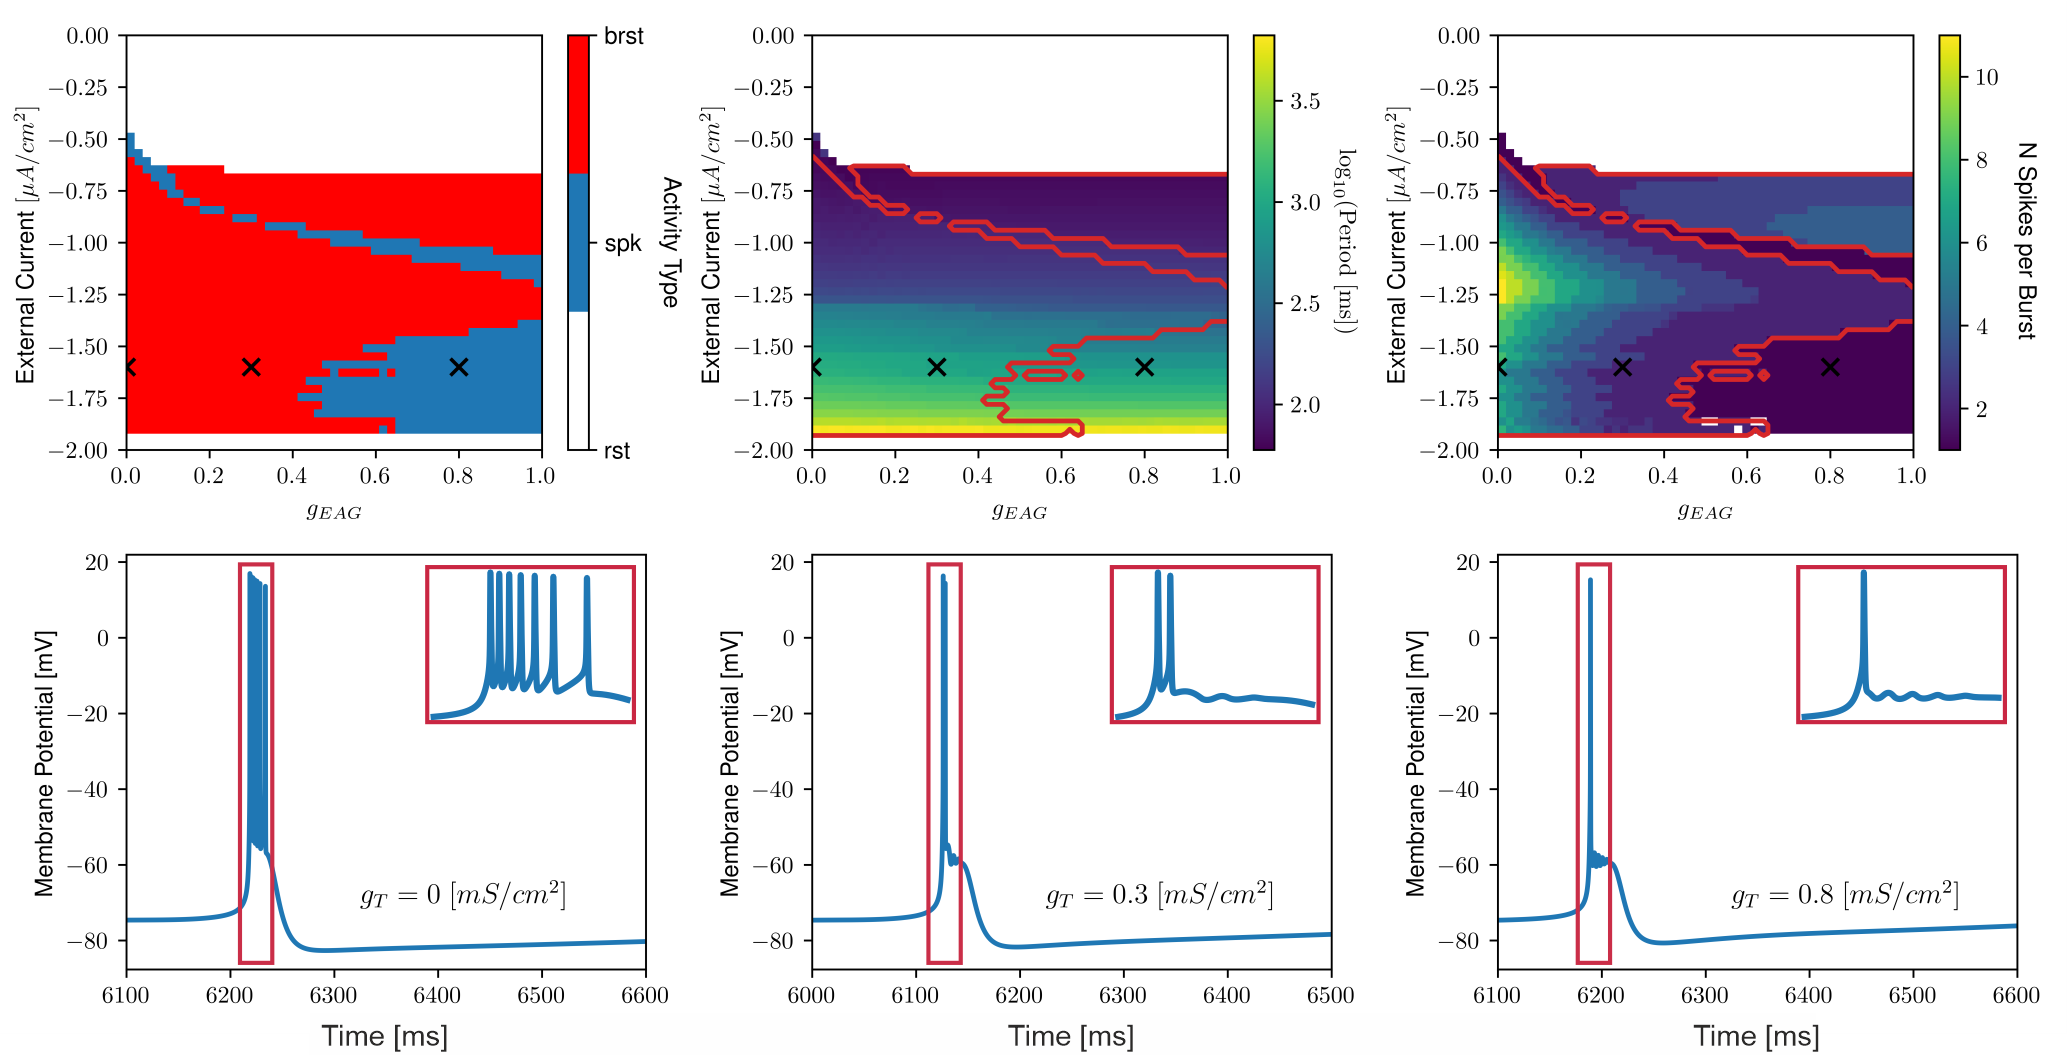
\includegraphics[width=\linewidth]{../img/spiking_to_bursting/transition_imshow.png}
    \caption[Spiking-to-Bursting Transition Induced by EAG Channels in Wang model]{
        \textbf{Spiking-to-Bursting Transition Induced by EAG Channels in Wang model}. \textcolor{red}{TEXT!!! + A-F. (A) Activity type; (B) Interburst period (here, tonic spiking is considered as one spike per burst), region where model showed two or more spikes per burst is outlied by red curve (corresponding to the red regions in (A); (C) number of spikes per burst); (D)-(F) examples of voltage traces in simulations. Corresponding parameter sets are denoted by "x" in (A)-(C). Insets shos the closeup of the spiking demonstrating that the number of spikes decreases with increasing $g_{EAG}$. For (D)-(F) the external input was set to $-1.6$ corresponding to the case when the model exhibits $1$Hz bursting.}
    }
    \label{fig:spiking_to_bursting_wang_phase_diagram}
\end{figure}

For fixed ecternal input, the number of spikes mainly decrease with increasing $g_{EAG}$ and
the firing pattern switches from bursting to tonic firing for a critical value of $g_{EAG}$, while the period remains relatively constant (Figure \ref{fig:spiking_to_bursting_wang_phase_diagram}A-C).
Figures \ref{fig:spiking_to_bursting_wang_phase_diagram}D-F further illustrate this effect by showing voltage traces from three representative simulations. The corresponding parameter combinations are indicated by 'x' in Figures \ref{fig:spiking_to_bursting_wang_phase_diagram}A-C.
Interestingly, there is a region in the phase space, where the number of spikes increase with increasing $g_{EAG}$ (Figure \ref{fig:spiking_to_bursting_wang_phase_diagram}C, upper boundary), however this region was not investigated within the scope of this thesis.

\textcolor{red}{The results obtained from other models were qualitatively similar and are therefore not included in the main text (see Figures ??? in the Appendix)}. 

\subsubsection{Bifurcation analysis} \label{subsubsec:spiking_to_bursting_bifurcation}

In the previous section it was demonstrated that \gls{eag} channel may be responsible for termination of the burst and the emergence of tonic spiking–like behavior in R5 neurons. This section investigates the underlying mechanisms through bifurcation analysis.

Figure \ref{fig:spiking_to_bursting_wang_bifurcation} presents the bifurcation analysis results for the model proposed by Wang \parencite{wangMultipleDynamicalModes1994}, which generates bursting behavior mediated by T-type $Ca^{2+}$ channels. In this model, the activation gate of the T-type channel is treated as instantaneous (see Section \ref{appendix:functions_and_parameters} for details), and the slow dynamics are governed by the inactivation gate, denoted by the variable $h$.To investigate how bursting depends on this variable, $h$ was treated as a bifurcation parameter, while all other varialbes were allowed to evolve freely. 

The analysis was performed for three representative values of $g_{EAG}$ corresponding to the 'x' markers in Figure \ref{fig:spiking_to_bursting_wang_phase_diagram}A-C. For each value of h, the stable and unstable fixed points were computed using \textsc{AUTO-07p}, along with the locations of Hopf and saddle-node (\gls{sn}) bifurcations. In Figure \ref{fig:spiking_to_bursting_wang_bifurcation}, stable and unstable fixed points are shown as solid and dashed black lines, respectively. Hopf bifurcations are indicated by circles, and saddle-node bifurcations by triangles. Periodic orbits were numerically continued from the Hopf bifurcations. The bursting trajectory was obtained by numerical simulations of the full system. Projection of the trajectory on $V$-$h$ plane is overlaid as a green curve. The direction of the trajectory is indicated by black arrow at the bottom of the plots.

Figure \ref{fig:spiking_to_bursting_wang_bifurcation}A shows results in the absence of the \gls{eag} channels. The analysis is similar to the fast-slow decomposition discussed in Section \ref{subsec:bifurcation_analysis}. The analysis follows a fast–slow decomposition similar to that described in Section \ref{subsec:bifurcation_analysis}. However, before discussing the results, an important aspect should be highlighted.

\vspace*{0.3cm}
\noindent\textbf{Effect of another slow variable on fast-slow decomposition}

From the perspective of fast-slow analysis, one might expect the full-system trajectory to closely follow the manifold of stable fixed points of the fast subsystem. However, the model contains an additional variable with a relatively slow timescale, associated to the \gls{hcn} channels (\textcolor{red}{see Section ??? for the corresponding parameters}). As discussed in Section \ref{subsubsec:ion_channel_contributions}, \gls{hcn} channels (referred to as "sag current" in \parencite{wangMultipleDynamicalModes1994}) are hyperpolarization-activated channels that mediate depolarizing current, thus, they contribute to dynamics at relatively low values of membrane potential.

\begin{figure}[!t]
    \centering
    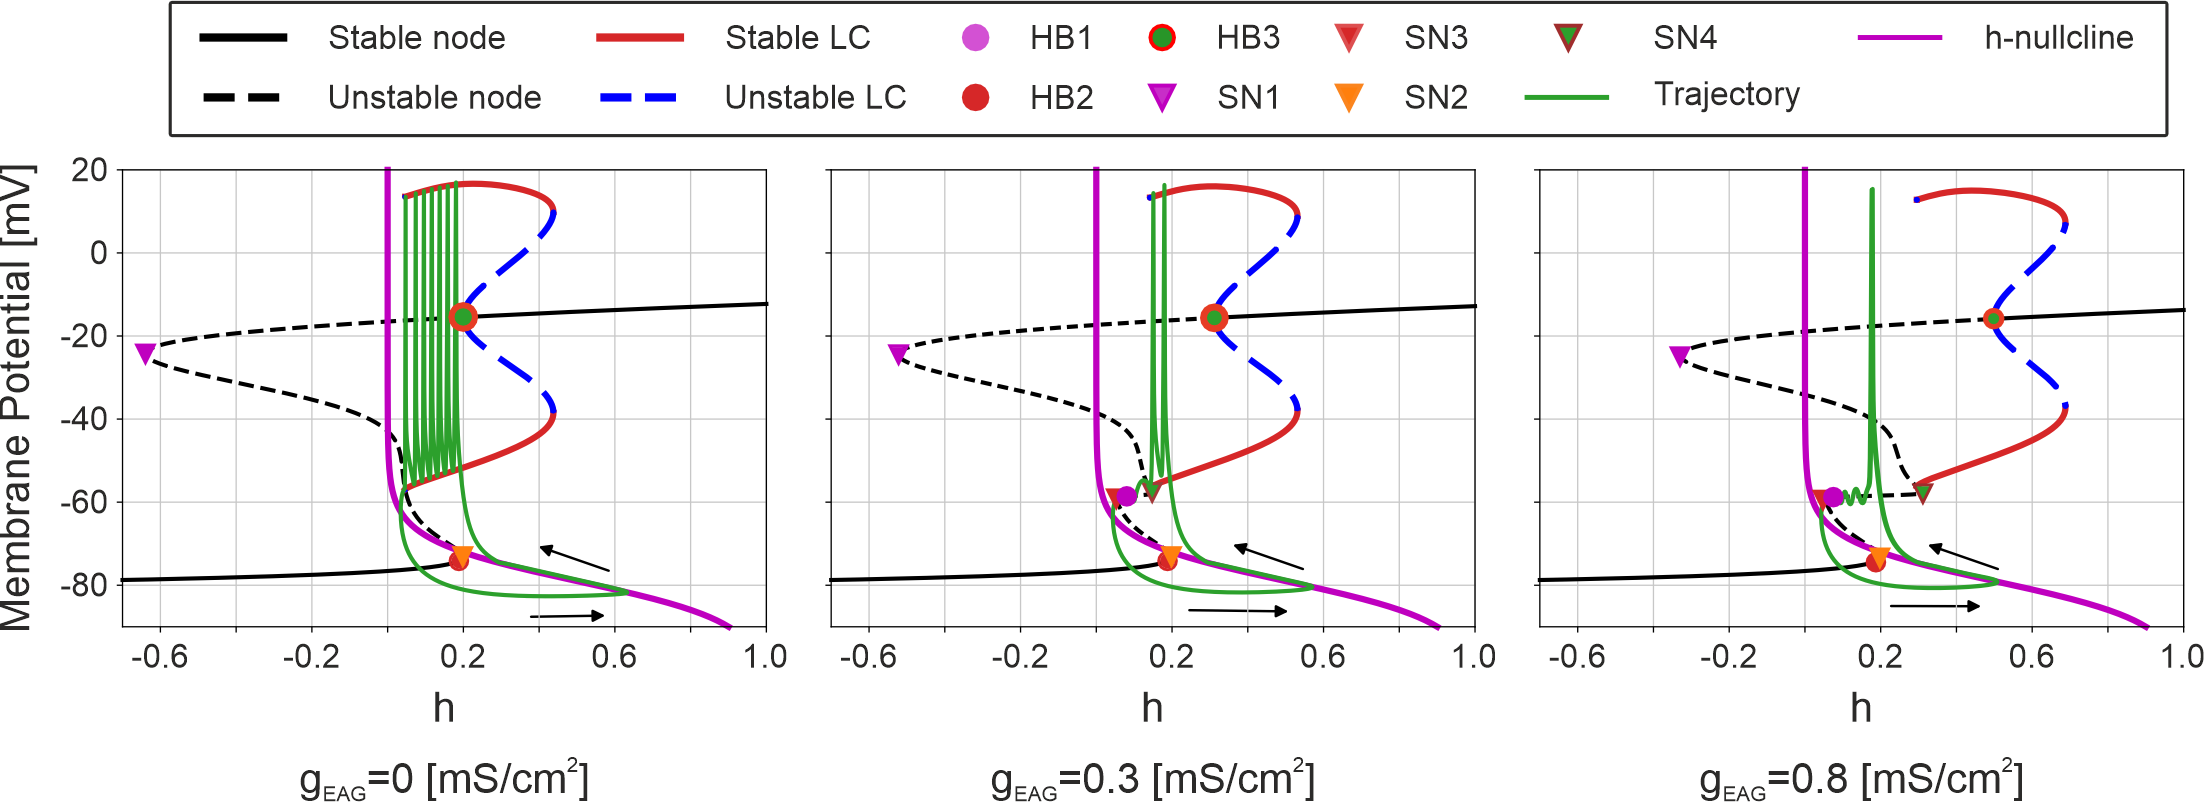
\includegraphics[width=\linewidth]{../img/spiking_to_bursting/bifurcation_wang.png}
    \caption[Transition from Spiking to Bursting via EAG channels]{
        \textbf{Transition from Spiking to Bursting via EAG channels}. \textcolor{red}{TEXT!!! + Make circles larger + A-C}
    }
    \label{fig:spiking_to_bursting_wang_bifurcation}
\end{figure}

\begin{figure}[!t]
    \centering
    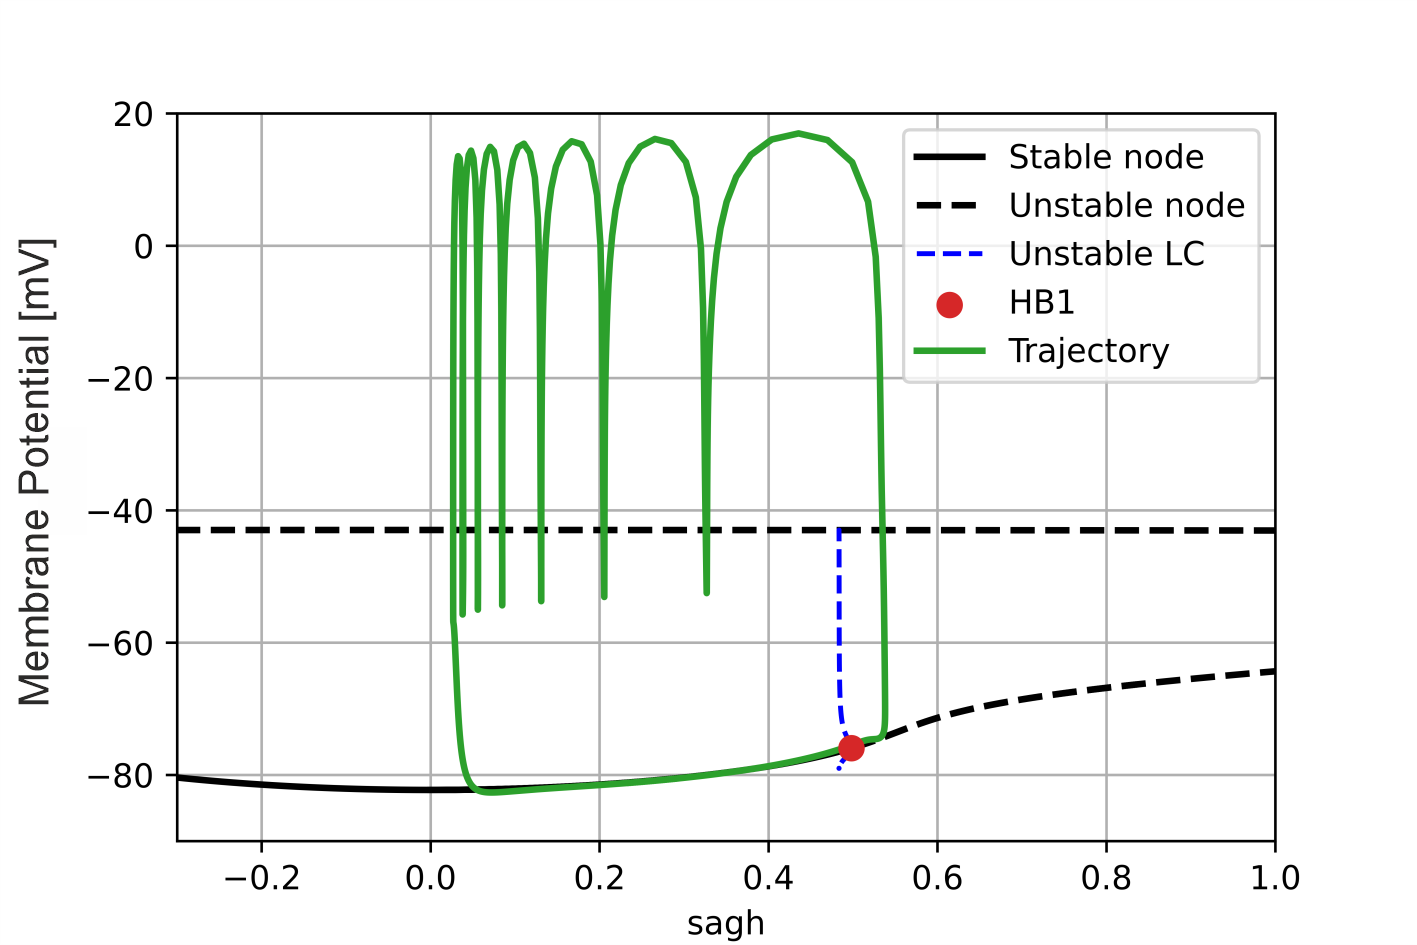
\includegraphics[width=0.6\linewidth]{../img/spiking_to_bursting/bifurcation_wang_sagh.png}
    \caption[Bifurcation Diagram - Wang Model with Sag Activation as Bifurcation Parameter]{
        \textbf{Bifurcation Diagram - Wang Model with Sag Activation as Bifurcation Parameter}. \textcolor{red}{TEXT!!!}
    }
    \label{fig:spiking_to_bursting_wang_bifurcation_sagh}
\end{figure}

Notably, \gls{hcn} channels contribute less during spiking phase. For example, at $-55$mV (approximately trough of the oscillation), the steady state activation has a value of $\sim 0.12$, decreasing to $\sim 0.06$ at $-50$mV and to $\sim 0.016$ at $-40$mV. Consequently, during spiking phase, the system behaves more like as the fast-slow in contrast to the resting state. This may explain why the bifurcation diagram seems to be more accurate in the spiking phase than in the resting phase of the reduced ("fast") subsystem without the $h$ variable. Indeed, when the activation variable of the \gls{hcn} channel was treated as a bifurcation parameter, the resulting trajectory closely followed the manifold of stable fixed points in the reduced subsystem where the \gls{hcn} activation was held constant (Figure \ref{fig:spiking_to_bursting_wang_bifurcation_sagh}).

To summarize, the transition of interest is from spiking to resting state, as \gls{eag} channels are considered to terminate bursts. Since the above analysis effectively captures the dynamics during the spiking phase, the approach remains suitable for investigating the mechanism.

\vspace*{0.3cm}
\noindent\textbf{Saddle-homoclinic orbit bifurcation underlies spiking-resting transition in Wang model}

As shown in Figure \ref{fig:spiking_to_bursting_wang_bifurcation}A, the spiking phase is deminished when the stable limit cycle (indicated by solid red lines) collides with unstable node (dashed black lines). This is commonly referred to as saddle-homoclinic orbit bifurcation \parencite{izhikevichDynamicalSystemsNeuroscience2006,izhikevichNEURALEXCITABILITYSPIKING2000} (see also Section \ref{subsec:bifurcation_analysis}).

In the absence of \gls{eag} channels the trajectory is attracted by the stable limit cycle after the resting state of the reduced system (i.e. one without the $h$ variable) looses stability, causing transition of the system to the spiking state. In spiking state, membrane potential provides a negative feedback to the variable $h$ (note, that inactivation gate of T-type channels closes at depolarized potentials; see steady state inactivation function for the $h$ gate in Figure \ref{fig:kinetic_plots_wang1994}).

As $g_{EAG}$ increases, the bifurcation point of the resting state remains unchanged (compare the onset of the bursts in Figure \ref{fig:spiking_to_bursting_wang_bifurcation}A-C). However, the point at which the limit cycle collides with the unstable nodes shifts to the right, and the system spends less time in the spiking regime. \color{orange} After $g_{eag}$ reachis a critical value, the limit cycle disappears, and the system returns to the resting state via saddle-homoclinic orbit after a single spike. \color{black}

\textcolor{red}{Look at Bifurcation in Codim-2 ???}

\textcolor{red}{Why is the curve shifting to the right? - Plot steady steady state I(V) plot for the "fast" subsystem + external current (horizontal line) for several values of $g_eag$. Their intersections will be fixed points. + two more line plots: one for I(V) of "fast" subsystem without $I_{eag}$ and another for $I_{eag}$ to visually see how I(V) is obtained from these two components}.

\end{document}